\paragraph{QuizziPedia::Front-End::Views::SignUpView}

\label{QuizziPedia::Front-End::View::SignUpView}
\begin{figure} [ht]
	\centering
	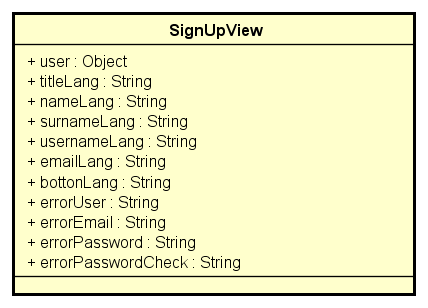
\includegraphics[scale=0.80]{UML/Classi/Front-End/QuizziPedia_Front-end_Views_SignUpView.png}
	\caption{QuizziPedia::Front-End::Views::SignUpView}
\end{figure} \FloatBarrier
\begin{itemize}
	\item \textbf{Descrizione}: view contenente le form dedicate alla registrazione utente. Contiene inoltre un link alla pagina di login;
	\item \textbf{Utilizzo}: permette all'utente di registrarsi al sistema inserendo i campi dati necessari;
	\item \textbf{Relazioni con altre classi}:
	\begin{itemize}
		\item \textbf{IN \texttt{SignUpModelView}}: classe di tipo modelview la cui istanziazione è contenuta all'interno della variabile di ambiente \$scope di . All'interno di essa sono presenti le variabili e i metodi necessari per il \textit{Two-Way Data-Binding\ped{G}} tra la view \texttt{SignUpView} e il controller \texttt{SignUpController};
		\item \textbf{IN \texttt{LangModel}}: rappresenta il modello delle informazioni per la giusta traduzione dell'applicazione.
	\end{itemize}
	\item \textbf{Attributi}:
	\begin{itemize}
		\item \texttt{+ user: Object} \\ Campo dati contenente i seguenti attributi: \texttt{name: String}, \texttt{surname: String}, \texttt{username: String}, \texttt{email: String}, \texttt{password: string} , \\ \texttt{passwordCheck: String};
		\item \texttt{+ titleLangSignUp: String} \\ Attributo che viene utilizzato per visualizzare la giusta traduzione del titolo della pagina, in italiano o in inglese;
		\item \texttt{+ nameLangSignUp: String} \\ Attributo che viene utilizzato per visualizzare la giusta traduzione della \textit{label\ped{G}} per l'inserimento del nome, in italiano o in inglese;
		\item \texttt{+ surnameLangSignUp: String} \\ Attributo che viene utilizzato per visualizzare la giusta traduzione della \textit{label\ped{G}} per l'inserimento del cognome, in italiano o in inglese;
		\item \texttt{+ usernameLangSignUp: String} \\ Attributo che viene utilizzato per visualizzare la giusta traduzione della \textit{label\ped{G}} per l'inserimento del nome utente, in italiano o in inglese;
		\item \texttt{+ emailLangSignUp: String} \\ Attributo che viene utilizzato per visualizzare la giusta traduzione della \textit{label\ped{G}} per l'inserimento della posta elettronica, in italiano o in inglese;
		\item \texttt{+ buttonLangSignUp: String} \\ Attributo che viene utilizzato per visualizzare la giusta traduzione della \textit{label\ped{G}} per il bottone di registrazione, in italiano o in inglese;
		\item \texttt{+ loginButtonLangSignUp: String} \\ Attributo che viene utilizzato per visualizzare la giusta traduzione della \textit{label\ped{G}} per il bottone di link all'autenticazione, in italiano o in inglese;
		\item \texttt{+ successSignUp: String} \\ Attributo che visualizza un messaggio di avvenuta registrazione;
		\item \texttt{+ errorUser: String} \\ Attributo che visualizza un eventuale messaggio di errore nell'inserimento della username;
		\item \texttt{+ errorEmail: String} \\ Attributo che visualizza un eventuale messaggio di errore nell'inserimento della email;
		\item \texttt{+ errorPassword: String} \\ Attributo che visualizza un eventuale messaggio di errore nell'inserimento della password;
		\item \texttt{+ errorPasswordCheck: String} \\ Attributo che visualizza un eventuale messaggio di errore nell'inserimento della password di conferma.
	\end{itemize}
\end{itemize}